\documentclass[../main.tex]{subfiles}
\begin{document}

    \textbf{Idea przepływu produktu przez system, podczas którego systematycznie zwiększana jest jego wartość.}\\

    Manifesto for Agile Software Development:
    \begin{itemize}
        \item Individuals and interactions $\rightarrow$ Teamwork and responsibility
        \item Working software $\rightarrow$ Business value
        \item Customer collaboration $\rightarrow$ Partnership elaboration
        \item Respodning to change $\rightarrow$ Prepare for change
    \end{itemize}

    Lightweight (XP, Scrum) or fuller (DSDM, AUP) approaches.

    \subsection{Programowanie ekstremalne - XP}
    Projekt informatyczny - \textbf{szczelny systemem czterech zmiennych: daty dostarczenia, kosztu, liczby
    defektów oraz niekompletności funkcji}.

    \begin{table}[H]
        \begin{center}
            \begin{tabular}{ c c }
                \raisebox{-\totalheight}{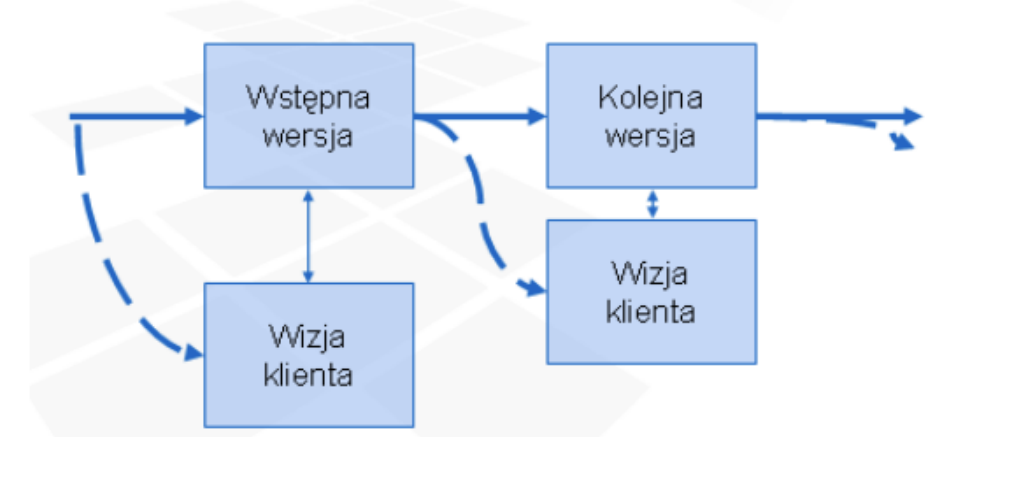
\includegraphics[width=0.5\textwidth]{model_xp.png}}
                &
                \raisebox{-\totalheight}{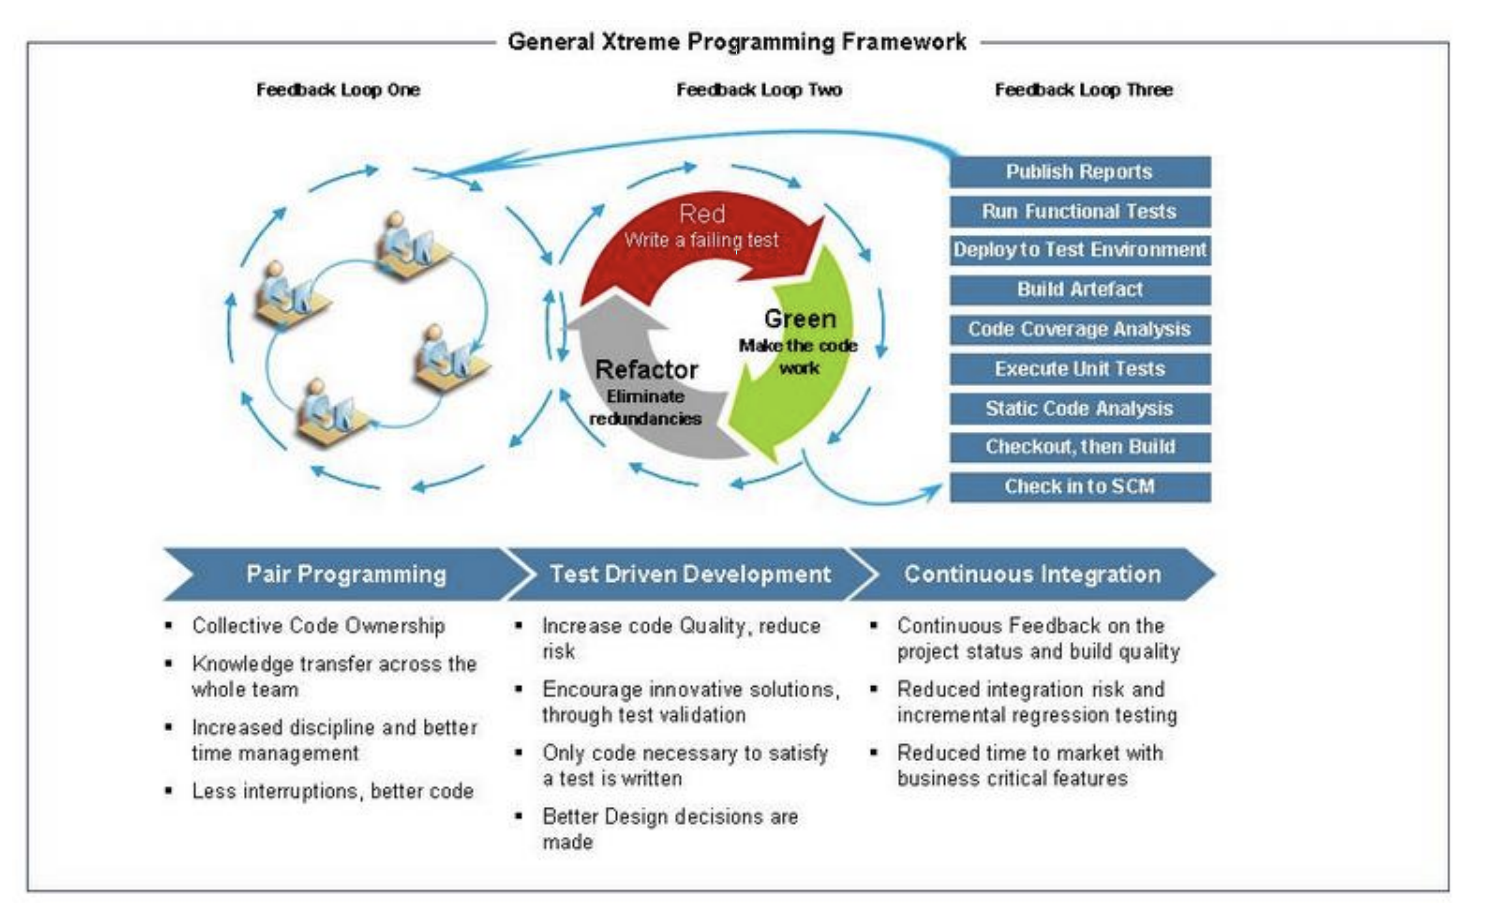
\includegraphics[width=0.5\textwidth]{xp_framework.png}}
                \\
            \end{tabular}
        \end{center}
    \end{table}

    \begin{itemize}
        \item brak fazy projektowania i dokumentacji,
        \item krótka perspektywa planowania,
        \item silne założenie, że klient pracuje cały czas z zespołem.
    \end{itemize}

    \textbf{Wartości}
    \begin{itemize}
        \item \textbf{Komunikacja} - przede wszystkim werbalna.
        \item \textbf{Prostota} - rozpoczynamy od najprostszego rozwiązania, spełniającego
        wymagania; refaktoryzacja pozwala na adaptacje oprogramowania do zmian.
        \item \textbf{Sprzężenie zwrotne} - obejmuje kilka aspektów (system, klient, zespół).
        \item \textbf{Odwaga} - potrzebna by: od razu produkować kod; refaktoryzować; wyrzucić zbędny kod.
        \item \textbf{Szacunek} - do pracy i czasu innych; między członkami zespołu.
    \end{itemize}

    \begin{table}[H]
        \begin{center}
            \begin{tabular}{ p{8cm} p{8cm} }
                \textbf{Struktura zespołu}
                &
                \begin{itemize}
                    \item \textbf{Role podstawowe}: programiści, klient,
                    \item \textbf{Role pomocnicze}: tester, coach, tracker.
                \end{itemize}
                \\

                \cmidrule(r){1-1}\cmidrule(l){2-2}
                \textbf{User Stories}
                &
                \begin{itemize}
                    \item opisują \textbf{funkcje systemu} z punktu widzenia użytkownika,
                    \item ważne by miały wartość dla klienta,
                    \item powinny być testowane.
                \end{itemize}
                \\

                \cmidrule(r){1-1}\cmidrule(l){2-2}
                \textbf{Gra planistyczna}
                &
                \begin{itemize}
                    \item \textit{pisanie} user story (klient),
                    \item \textit{oszacowanie} user story (informatycy),
                    \item \textit{dzielenie} user story/wybór zakresu iteracji (klient).
                \end{itemize}
                \\

                \cmidrule(r){1-1}\cmidrule(l){2-2}
                \textbf{Zapewnianie jakości}
                &
                \begin{itemize}
                    \item prostota,
                    \item unikanie optymalizacji,
                    \item Test Driven Development - TTD,
                    \item automatyczne testowanie,
                    \item refaktoryzacja.
                \end{itemize}
                \\

                \cmidrule(r){1-1}\cmidrule(l){2-2}
                \textbf{Testy akceptacyjne}
                &
                \begin{itemize}
                    \item pochodzą od klienta (w ten sposób dokładnie określa,
                    zachowanie systemu),
                    \item najlepiej gdy mogą być wykonywane automatycznie (tester).
                \end{itemize}
                \\

                \cmidrule(r){1-1}\cmidrule(l){2-2}
                \textbf{Programowanie parami}
                &
                \begin{itemize}
                    \item zaleca się, by całość kodu pisana była w parach,
                    \item częste zmiany w parach,
                    \item wspólny standard kodowania,
                    \item kod jest własnością całego zespołu,
                    \item niezbędny system kontroli wersji.
                \end{itemize}
                \\
            \end{tabular}
        \end{center}
    \end{table}

    \subsection{SCRUM}
    Metoda przy użyciu której ludzie mogą z powodzeniem rozwiązywać \textbf{złożone problemy
    adaptacyjne}, by w sposób produktywny i kreatywny wytwarzać produkty o najwyższej możliwej wartości.
    \begin{itemize}
        \item lekki;
        \item łatwy do zrozumienia;
        \item bardzo trudny do opanowania.
    \end{itemize}

    \textbf{Trzy filary} teorii SCRUMa:
    \begin{itemize}
        \item \textbf{Adaptacja} - powinna być \underline{ciągła}. Korekta musi być
        wykonana jak najszybciej, by ograniczyć dalsze następstwa problemów.
        \item \textbf{Przejrzystość} - wszystkie \underline{istotne aspekty} procesu
        muszą być \underline{widoczne} dla osób odpowiedzialnych za osiągane rezultaty.
        \item \textbf{Inspekcja} – poddawane \underline{regularnej} inspekcji są zarówno scrumowe
        artefakty jak i postępy prac.
    \end{itemize}

    \subsubsection{Role}
    \begin{table}[H]
        \begin{center}
            \begin{tabular}{ p{.5\textwidth} p{0.5\textwidth} }
                \textbf{Właściciel Produktu}
                &
                \begin{itemize}
                    \item odpowiedzialny za maksymalizację wartości produktu i pracy Zespołu
                    Deweloperskiego,
                    \item jedyną osoba zarządzająca Rejestrem Produktu, tzn:
                    \begin{itemize}
                        \item jasne artykułowanie elementów Rejestru Produktu, określanie
                        ich kolejności w sposób zapewniający osiąganie założonych celów i misji;
                        \item zapewnianie dostępności i przejrzystości Rejestru Produktu dla wszystkich i to, że dobrze opisuje czym
                        Zespół Scrumowy będzie się zajmował.
                    \end{itemize}
                \end{itemize}
                \\

                \cmidrule(r){1-1}\cmidrule(l){2-2}
                \textbf{Zespoł deweloperski}
                &
                \begin{itemize}
                    \item złożony z profesjonalistów (3-9 osób); samoorganizujący się, wielofunkcyjny.
                    \item ma za zadanie dostarczenie (na zakończenie
                    każdego Sprintu), gotowego do wydania Przyrostu produktu,
                    \item nie przewiduje tytułów innych niż „Deweloper”,
                    \item odpowiedzialność za wykonywaną pracę ponosi cały Zespół; brak podziału na podzespoły.
                \end{itemize}
                \\

                \cmidrule(r){1-1}\cmidrule(l){2-2}
                \textbf{Scrum Master}
                &
                \begin{itemize}
                    \item odpowiedzialny za to, by Scrum był rozumiany i stosowany,
                    \item upewnia się, że Zespół Scrumowy stosuje się do założeń teorii Scruma, jego praktyk i reguł postępowania.
                    \item wspiera zarówno Właściciela Produktu, jak i Zespól Deweloperski.
                \end{itemize}
                \\
            \end{tabular}
        \end{center}
    \end{table}

    \subsubsection{Artefakty}
    \begin{table}[H]
        \begin{center}
            \begin{tabular}{ p{.5\textwidth} p{0.5\textwidth} }
                \textbf{Rejestr Produktu}
                &
                uporządkowana lista wszystkiego,
                co może być potrzebne w produkcie oraz jedyne źródło wymaganych zmian.
                Odpowiedzialny za RP jest Właściciel Produktu.
                Elementy posiadają atrybuty: opis, kolejność i oszacowanie (estymację).
                \\

                \cmidrule(r){1-1}\cmidrule(l){2-2}
                \textbf{Rejestr Sprintu}
                &
                podzbiór elementów RP wybranych do Sprintu rozszerzony o plan
                dostarczenia Przyrostu produktu.
                RS definiuje pracę, jaką ZD wykona by przekształcić elementy
                RP w „Ukończony” Przyrost.
                RS jest dobrze widocznym, tworzonym w czasie rzeczywistym obrazem pracy, jaką ZD planuje wykonać w trakcie Sprintu.
                RS należy tylko i wyłącznie do ZD.
                \\

                \cmidrule(r){1-1}\cmidrule(l){2-2}
                \textbf{Monitorowanie postępów Sprintu}
                &
                możliwe w każdym momencie Sprintu (Codzienny Scrum).
                \\

                \cmidrule(r){1-1}\cmidrule(l){2-2}
                \textbf{Przyrost}
                &
                suma wszystkich elementów RP zakończonych podczas wszystkich spirntów.
                Na koniec Sprintu nowy Przyrost musi być „Ukończony”.
                \\

                \cmidrule(r){1-1}\cmidrule(l){2-2}
                \textbf{Definicja Ukończenia}
                &
                Aby zapewnić przejrzystość, wszyscy członkowie danego zespołu muszą mieć wspólne
                pojmowanie, co to znaczy, że praca jest skończona. W miarę dojrzewania Zespołu Scrumowego oczekuje się, że ich Definicja Ukończenia będzie
                zawierała coraz bardziej rygorystyczne kryteria zapewniania jeszcze wyższej jakości.
                \\
            \end{tabular}
        \end{center}
    \end{table}

    \subsubsection{Zdarzenia}
    \textbf{Cztery formalne punkty} (ograniczone czasowo, wprowadzajace regularność) przeprowadzania inspekcji i dokonania korekty (adaptacji) (każde oprócz Sprinut).


    \begin{table}[H]
        \begin{center}
            \begin{tabular}{ p{.4\textwidth} p{0.6\textwidth} }
                \textbf{Sprint} – serce Scruma
                &
                \begin{itemize}
                    \item stałe przez okres trwania prac ograniczenie czasowe ($\leq$ 1 mies)
                    \item podczas Sprintu wytwarzany jest Przyrost ukończonej,
                    używalnej i potencjalnie gotowej do wydania funkcjonalności,
                    \item niedozwolone są zmiany, które wpłyną na cel Sprintu,
                    \item niezmienny skład Zespołu Deweloperskiego i jego cel jakościowy.
                \end{itemize}
                \\

                \cmidrule(r){1-1}\cmidrule(l){2-2}
                \textbf{Przerwanie Sprintu}
                &
                \begin{itemize}
                    \item tylko Właściciel Produktu ma prawo to zrobić;
                    \item w przypadku dezaktualizacji celu Sprintu,
                    \item zużywa zasoby, bo powoduje przegrupowanie podczas kolejnego Planowania
                    Sprintu.
                \end{itemize}
                \\

                \cmidrule(r){1-1}\cmidrule(l){2-2}
                \textbf{Planowanie Sprintu} - 8h/mies
                &
                \begin{itemize}
                    \item Część pierwsza: \textit{Co będzie zrobione w tym Sprincie?}
                    Wejście:
                    \begin{itemize}
                        \item Rejestr Produktu;
                        \item ostatni przyrost;
                        \item przewidywana pojemność ZD;
                        \item ostatnie odczyty wydajności;
                    \end{itemize}
                    Wyjście:
                    \begin{itemize}
                        \item elementu Rejestru Produktu
                        wybrane do zaimplementowania;
                        \item cel Sprintu.
                    \end{itemize}
                    \item Część druga: \textit{Jak wybrana praca będzie wykonana?}
                    \begin{itemize}
                        \item zwykle rozpoczęcie od stworzenia projektu systemu i planu prac
                        niezbędnych do przetworzenia elementów Rejestru Produktu w działający Przyrost produktu.
                        \item zanim Planowanie Sprintu dobiegnie końca, ZD powinien móc wytłumaczyć Właścicielowi
                        Produktu i Scrum Masterowi, w jaki sposób ma zamiar pracować, organizując się samodzielnie, by osiągnąć Cel
                        Sprintu i wytworzyć oczekiwany Przyrost.
                    \end{itemize}
                \end{itemize}
                \\

                \cmidrule(r){1-1}\cmidrule(l){2-2}
                \textbf{Codzienny Scrum} - 15 min/d
                &
                \begin{itemize}
                    \item Co zostało wykonane od ostatniego potkania?
                    \item Co zostanie wykonane przed kolejnym spotkaniem?
                    \item Jakie przeszkody stoją na drodze?
                \end{itemize}
                \\

                \cmidrule(r){1-1}\cmidrule(l){2-2}
                \textbf{Przegląd Sprintu} - 4h na zakończenie Sprintu
                &
                \begin{itemize}
                    \item WP stwierdza, które funkcjonalności zostały
                    „Ukończone”, a które nie;
                    \item ZD omawia, co poszło dobrze w trakcie
                    Sprintu; jakie były problemy i jak je rozwiązano;
                    \item ZD prezentuje „Ukończoną” pracę i
                    odpowiada na pytania dotyczące Przyrostu,
                    \item WP omawia Rejestr Produktu w aktualnej
                    jego postaci. Przewiduje termin zakończenia prac.
                    \item Cala grupa omawia kolejne kroki.
                \end{itemize}
                \\

                \cmidrule(r){1-1}\cmidrule(l){2-2}
                \textbf{Retrospektywa Sprintu} - okazja do przeprowadzenia inspekcji
                swoich działań i opracowania planu usprawnień.
                &
                \begin{itemize}
                    \item Sprawdzenie, co działo się w ostatnim Sprincie, biorąc pod
                    uwagę ludzi, zależności, procesy i narzędzia;
                    \item Zidentyfikowanie i uporządkowanie istotnych elementów, które
                    sprawdziły się w działaniu oraz tych, które kwalifikują się do
                    poprawy;
                    \item Stworzenie planu wprowadzania w życie usprawnień sposobu
                    wykonywania pracy przez Zespół Scrumowy.
                \end{itemize}
                \\
            \end{tabular}
        \end{center}
    \end{table}


    \subsection{AGILE PM (DSDM Atern)}

    \begin{figure}[H]
        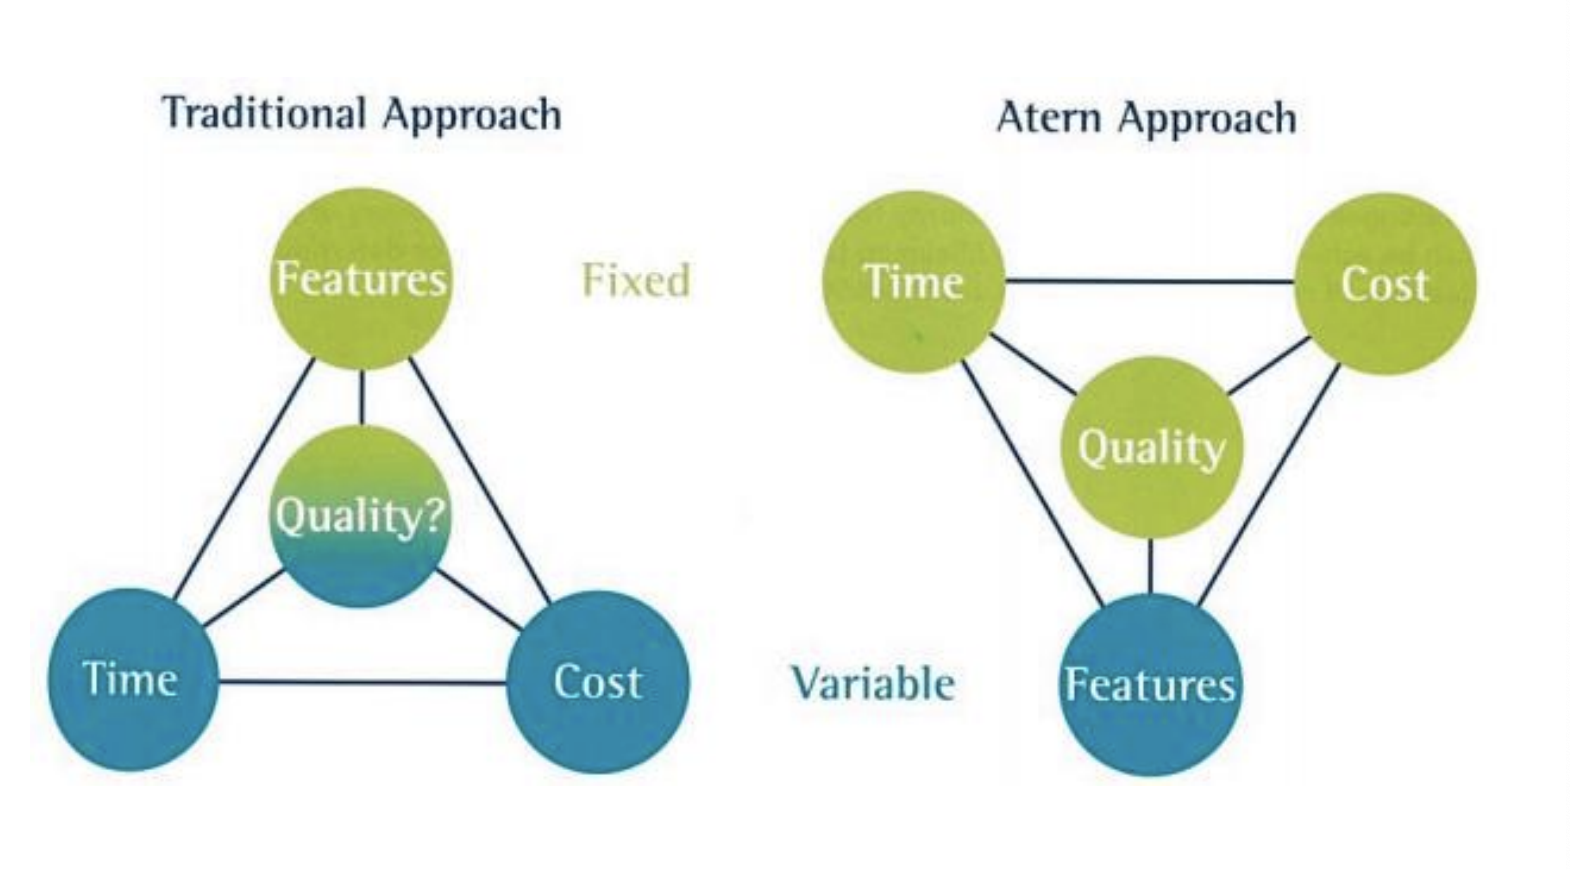
\includegraphics[width=\linewidth]{atern_approach.png}
    \end{figure}

    \textbf{PROCESS - PEOPLE - PRODUCTS - PRACTISES}
    \begin{itemize}
        \item Focus on the \textit{business need}
        \item Deliver \textit{on time}
        \item \textit{Collaborate}
        \item Never compromise \textit{quality}
        \item Build incrementally from \textit{firm foundations}
        \item Develop \textit{iteratively}
        \item \textit{Communicate continuously} and clearly
        \item Demonstrate \textit{control}
    \end{itemize}



    \subsubsection{Fazy projektu}
    \begin{figure}[H]
        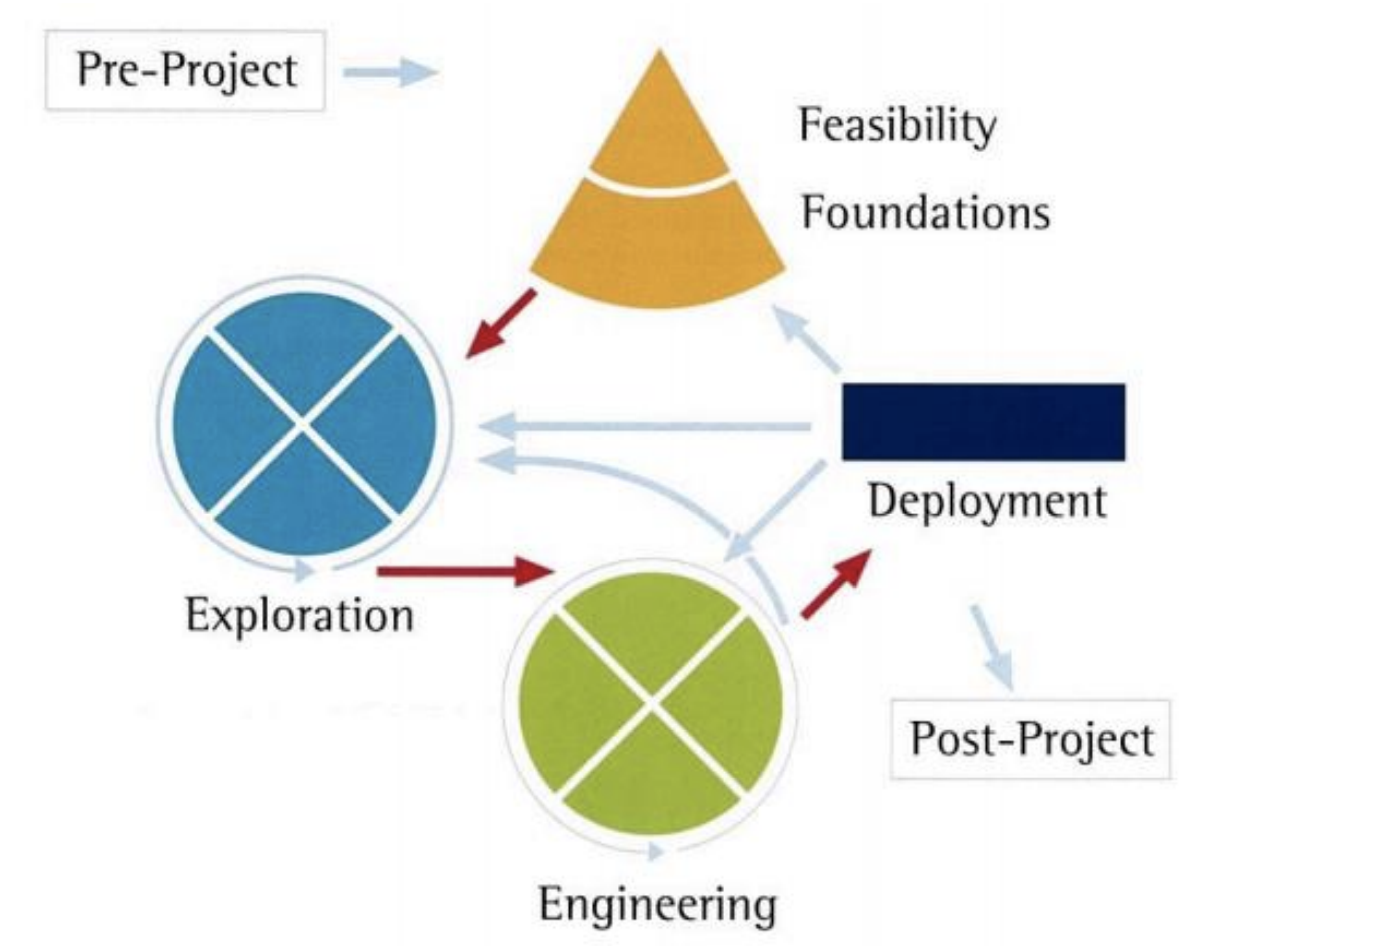
\includegraphics[width=\linewidth, height=10cm]{agile_fazy.png}
    \end{figure}


    \begin{table}[H]
        \begin{center}
            \begin{tabular}{ p{.3\textwidth} p{0.7\textwidth} }
                \textbf{Pre-project}
                &
                \begin{itemize}
                    \item problem biznesowy; identyfikacja Business Sponsor i Business Visionary,
                    \item zakres, plan i zasoby na fazę Feasibility.
                \end{itemize}
                \\

                \textbf{Feasibility}
                &
                \begin{itemize}
                    \item ustalić wykonalność rozwiązania problemu biznesowego,
                    \item identyfikacja potencjalnych zysków; zarys możliwych podejść do rozwiązania,
                    \item pierwsze estymaty czasowe i kosztowe.
                \end{itemize}
                \\

                \textbf{Foundation}
                &
                \begin{itemize}
                    \item wysoko poziomowe wymagania,
                    \item identyfikacja wspieranych procesów biznesowych,
                    \item podstawy architektury systemu; sposób zapewnienia wysokiej jakości.
                \end{itemize}
                \\

                \textbf{Exploration}
                &
                \begin{itemize}
                    \item uszczegóławianie wymagań; iteracyjnie działające rozwiązanie,
                    \item zarys możliwych podejść do rozwiązania.
                \end{itemize}
                \\

                \textbf{Engineering}
                &
                \begin{itemize}
                    \item rozwijanie rozwiązania z fazy Exploration.
                \end{itemize}
                \\

                \textbf{Deployment}
                &
                \begin{itemize}
                    \item potwierdzenie wydajności rozwiązania,
                    \item dostarczenie (iteracyjnie) rozwiązania,
                    \item dostarczenie potrzebnej dokumentacji.
                \end{itemize}
                \\
            \end{tabular}
        \end{center}
    \end{table}




    \subsubsection{Role}
    \begin{table}[H]
        \begin{center}
            \begin{tabular}{ p{.3\textwidth} p{0.7\textwidth} }
                \textbf{Business Sponsor}
                &
                \begin{itemize}
                    \item najwyższy rangą w projekcie; zapewnia finansowanie i zasoby,
                    \item właściciel tzw. przypadku biznesowego.
                \end{itemize}
                \\


                \textbf{Business visionary}
                &
                \begin{itemize}
                    \item definiuje wizję projektu i komunikuje ją,
                    \item ma zapewnić współprace na wszystkich poziomach projektu,
                    \item wkład w najważniejsze wymagania; arbiter w przypadku sporów.
                \end{itemize}
                \\

                \textbf{Project manager}
                &
                \begin{itemize}
                    \item monitoruje postęp projektu; motywuje zespoły, zatrudnia specjalistów,
                    \item wysoko poziomowe planowanie harmonogramu, zarządzanie ryzykiem w projekcie.
                \end{itemize}
                \\

                \textbf{Technical coordination}
                &
                \begin{itemize}
                    \item definiuje środowisko pracy,
                    \item doradza w sprawach technicznych, pilnuje standardów,
                    \item zajmuje się wymaganiami niefunkcjonalnymi.
                \end{itemize}
                \\

                \textbf{Team Leader}
                &
                \begin{itemize}
                    \item skupiony na zespole, pilnuje dostarczania poszczególnych komponentów na czas,
                    \item raportuje postęp do PM, prowadzi spotkania zespołowe.
                \end{itemize}
                \\

                \textbf{Business Ambassador}
                &
                \begin{itemize}
                    \item rola biznesowa w zespole deweloperskim,
                    \item dzieli się perspektywa biznesową z zespołem, dostarcza scenariusze biznesowe,
                    \item tworzy dokumentacje użytkownika.
                \end{itemize}
                \\

                \textbf{Business Analyst}
                &
                \begin{itemize}
                    \item komunikacja między biznesem a zespołem deweloperskim,
                    \item dystrybucja i wstępna akceptacja dokumentów biznesowych.
                \end{itemize}
                \\

                \textbf{Solution Developer}
                &
                \begin{itemize}
                    \item skupiony na dostarczeniu rozwiązania,
                    \item modele potrzebne do dostarczenia rozwiązania, dokumentacja.
                \end{itemize}
                \\

                \textbf{Solution Tester}
                &
                \begin{itemize}
                    \item definiuje scenariusze testowe, test casy,
                    \item komunikuje wyniki testów do TL, pracuje z BAs nad testami akceptacyjnymi.
                \end{itemize}
                \\

            \end{tabular}
        \end{center}
    \end{table}


    \subsubsection{Produkty}

    Levels of priority - \textbf{MoSCoW}
    \begin{itemize}
        \item \textbf{M}ust Have
        \item \textbf{S}hould Have
        \item \textbf{C}ould Have
        \item \textbf{W}on’t Have this time
    \end{itemize}

    Fazy \textbf{TIMEBOX}u:
    \begin{itemize}
        \item \textbf{Kick-off} – krótka sesja, która ma pomoc zrozumieniu celu timeboxa,
        \item \textbf{Investigation} – szczegóły wszystkich produktów, które mamy wykonać,
        \item \textbf{Refinement} – kodowanie i testowanie,
        \item \textbf{Consolidation} – spinanie całości.
    \end{itemize}

    \textbf{Iterative development}:
    \begin{itemize}
        \item \textbf{Identify}: zespół definiuje cel
        \item \textbf{Plan}: kto powinien zrobić co
        \item \textbf{Evolve}: wykonywanie
        zaplanowanych czynności
        \item \textbf{Review}: sprawdzanie rezultatów
    \end{itemize}


    \begin{figure}[H]
        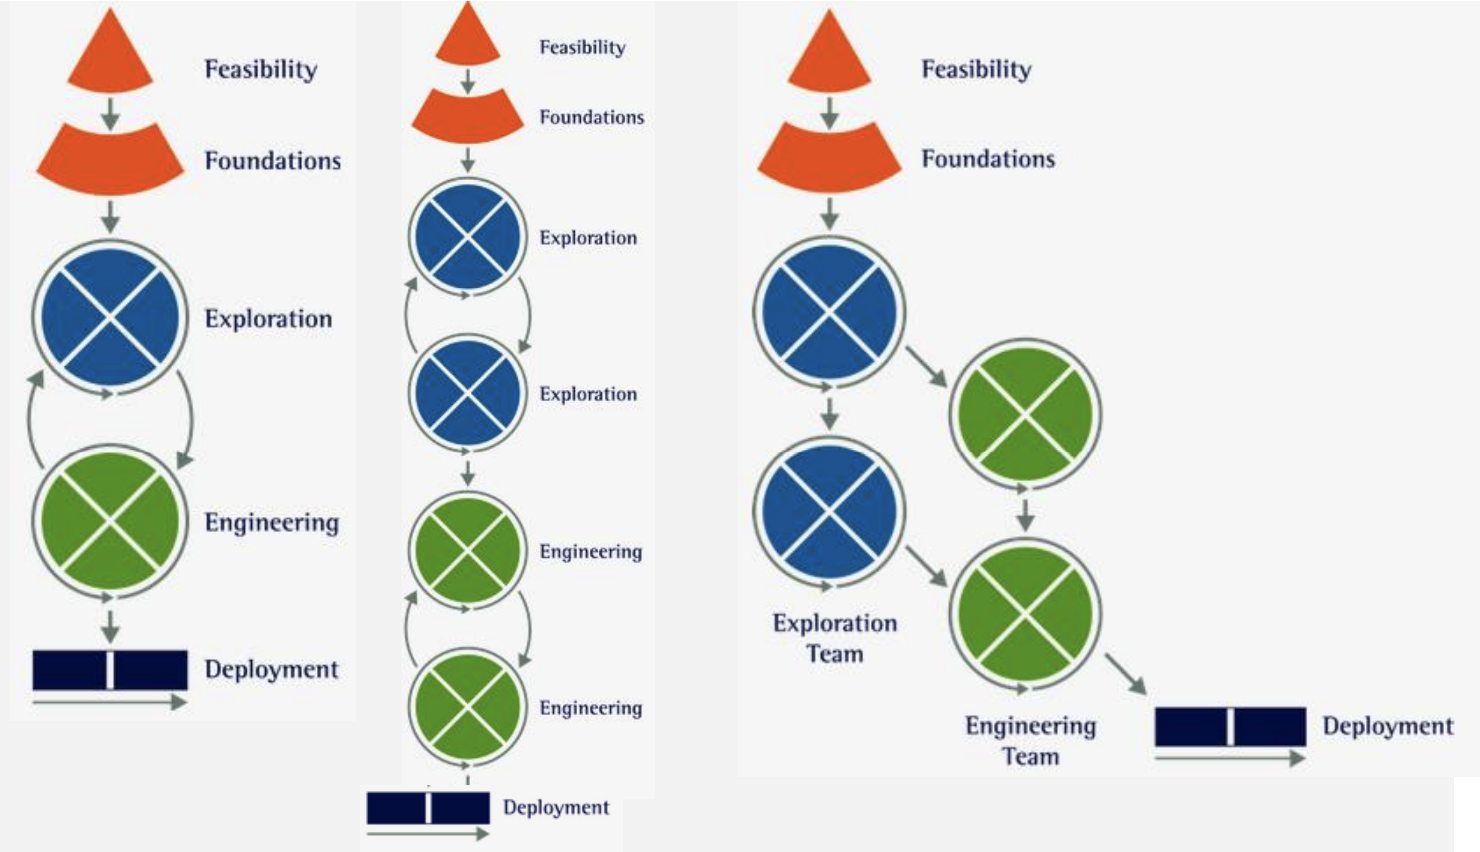
\includegraphics[width=\linewidth]{agile_iterations.png}
    \end{figure}


    \subsection{AUP - Agile Unified Process}

    \begin{itemize}
        \item uproszczona wersja Rational Unified Process,
        \item stosuje zwinne techniki takie jak TDD, refactoring,
        \item \textbf{seryjny w dużej skali, iteracyjny w małej}.
    \end{itemize}

    \begin{table}[H]
        \begin{center}
            \begin{tabular}{ c p{8cm} }
                \raisebox{-\totalheight}{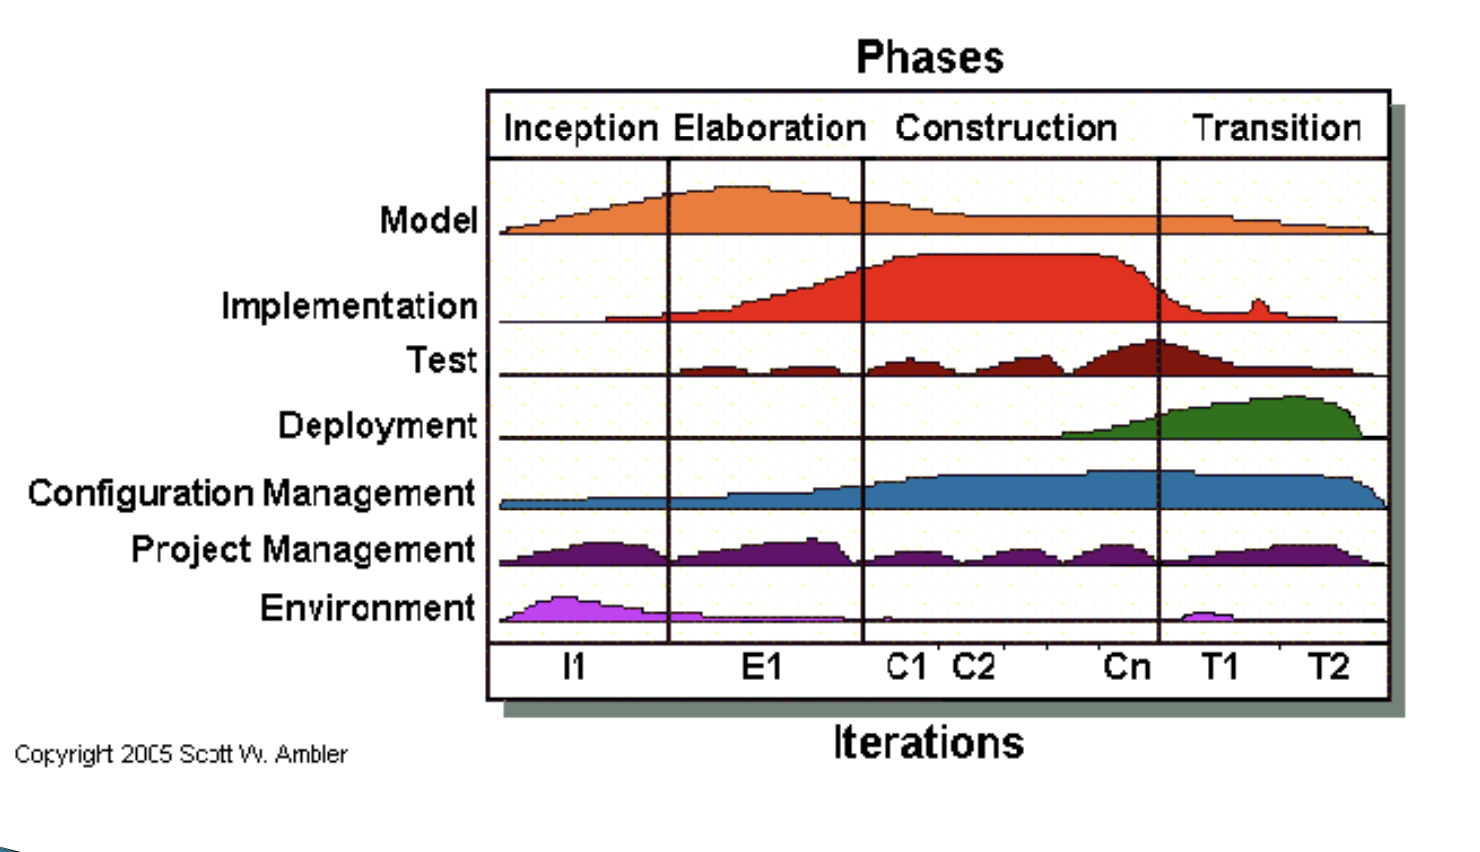
\includegraphics[width=0.5\textwidth]{aup_phases.png}}
                &
                \textbf{Zasady AUP}
                \begin{itemize}
                    \item twój zespół wie, co robi;
                    \item prostota;
                    \item zwinność;
                    \item skupienie się na istotnych aktywnościach;
                    \item niezależność od narzędzi;
                    \item możliwość adaptacji.
                \end{itemize}
                \\
            \end{tabular}
        \end{center}
    \end{table}



    \subsection{KANBAN}

    \begin{table}[H]
        \begin{center}
            \begin{tabular}{ c p{8cm} }
                \raisebox{-\totalheight}{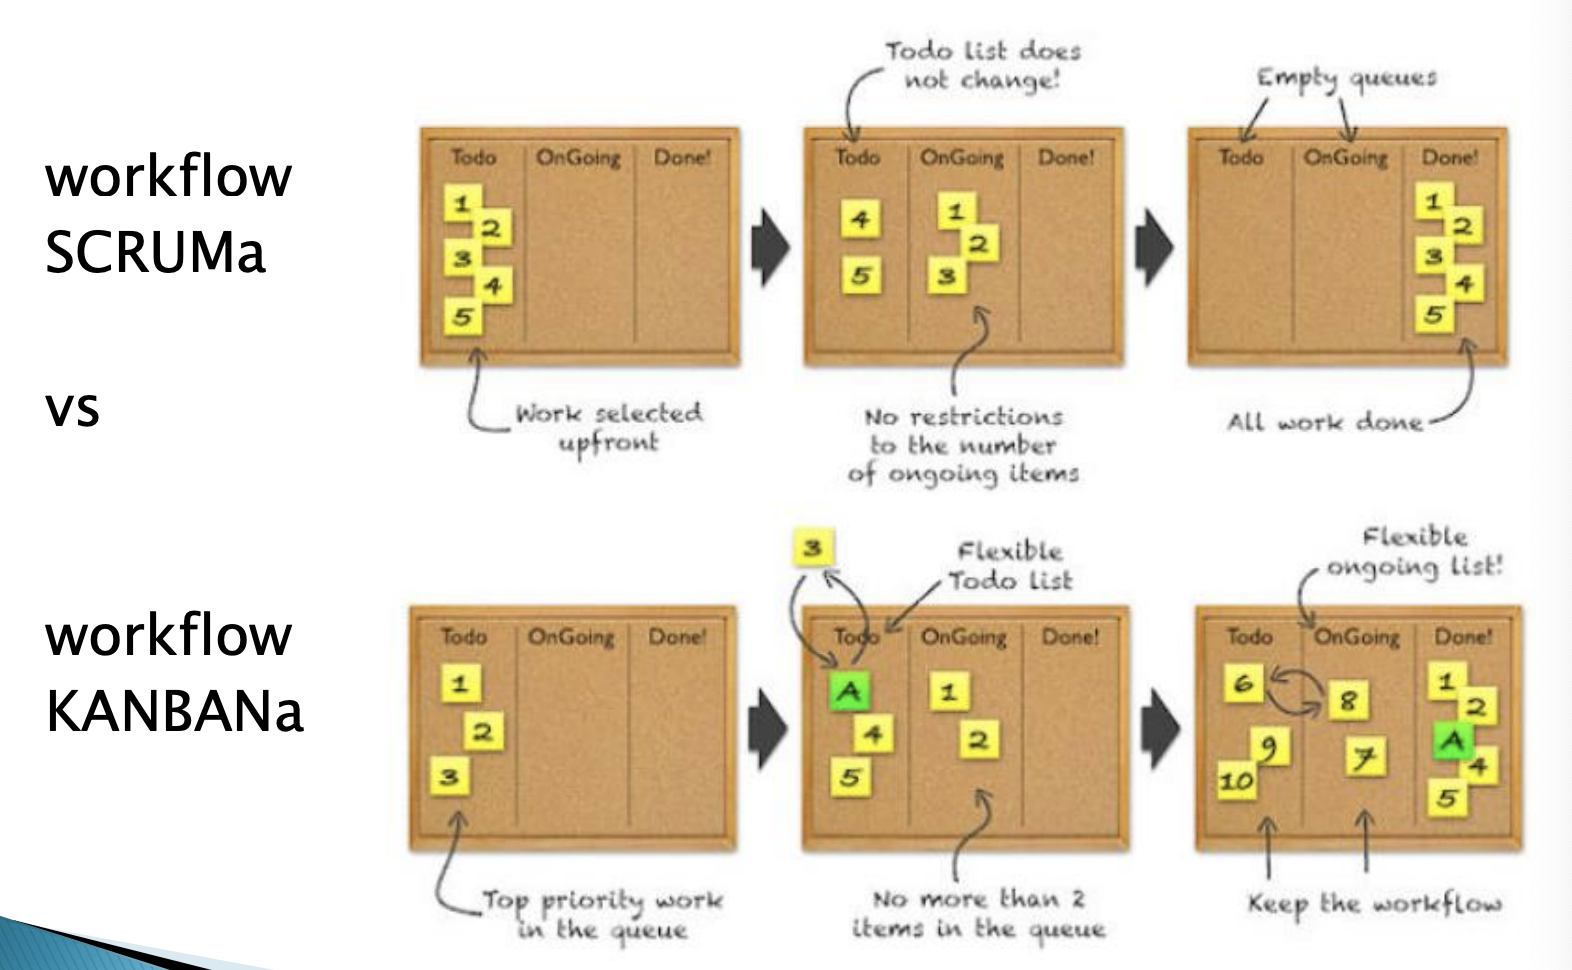
\includegraphics[width=0.5\textwidth]{kanban_vs_scrum.png}}
                &
                \begin{itemize}
                    \item \textbf{ciągły przepływ produktu przez system produkcyjny}.
                    \item podstawa systemów produkcyjnych Toyoty i pochodnych
                    \item \textbf{system pull} sterowany
                    jest przez \textbf{składane przez odbiorcę zamówienie}, a nie ogólny, arbitralny plan produkcji.
                    \item odnosi się do \textbf{etapowości procesu wytwarzania
                    oprogramowania}, przynajmniej trzy stany pracy — do zrobienia, w trakcie, gotowe.
                \end{itemize}
                \\
            \end{tabular}
        \end{center}
    \end{table}

    \textbf{Sześć reguł kanbana}:
    \begin{itemize}
        \item odbiorca przetwarza dokładnie tyle elementów, ile opisane
        jest na karcie kanban;
        \item dostawca wytwarza dokładnie tyle elementów, ile opisane jest
        na karcie kanban;
        \item żaden element nie jest wytwarzany lub przekazywany
        pomiędzy stanowiskami bez karty kanban;
        \item karta kanban musi towarzyszyć każdemu elementowi czy
        półproduktowi przetwarzanemu w ramach systemu;
        \item elementy wadliwe lub występujące w niewłaściwych ilościach,
        nigdy nie są przekazywane w dół procesu;
        \item limity obowiązujące na każdym z etapów (fizyczna ilość kart
        kanban) są stopniowo obniżane aby redukować zapasy i
        odkrywać nieefektywności procesów produkcji, dążąc do ich
        doskonalenia.
    \end{itemize}

    \subsubsection{Kanban vs Scrum}

    \begin{table}[H]
        \begin{center}
            \begin{tabular}{ | p{8cm} p{8cm} |}
                \toprule
                \multicolumn{2}{| p{16cm} |}{\textbf{Sposób pracy}}\\
                \toprule
                \textbf{Scrum} & \textbf{Kanban}\\
                \toprule

                Rytmiczność pracy & Płynność pracy\\
                \cmidrule(r){1-1}\cmidrule(l){2-2}
                Synchronizacja aktywnowści & Aktywności synchroniczne lub asynchronicznie\\
                \cmidrule(r){1-1}\cmidrule(l){2-2}
                Skupienie na celu, minimalizacja przełączania między zadaniami
                &
                Niski czas odpowiedzi systemu na zmiany\\
                \cmidrule(r){1-1}\cmidrule(l){2-2}
                Pewność realizacji aktywności związanych z Agile SD
                &
                Możliwość doboru czynności dopasowanych do środowiska\\
                \cmidrule(r){1-1}\cmidrule(l){2-2}
                Pełne zaangażowanie zespołu, wiedza ogólna i współodpowiedzialność
                &
                Możliwość pełnego wykorzystania specjalistów\\
                \cmidrule(r){1-1}\cmidrule(l){2-2}
                Trudność w pełnym wykorzystaniu zespołu ze względu na skokowy sposób pracy
                &
                Możliwość pełnego wykorzystania zespołu ze względu na płynny sposób pracy\\
                \cmidrule(r){1-1}\cmidrule(l){2-2}
                Niebezpieczeństwo przeładowania poprzez stosowanie źle wyznaczonych miar podczas planowania,
                penalizacji związanej z niedostarczeniem funkcjonalności
                &
                Niebezpieczeństwo przeładowania poprzez nadmierną optymalizację wykorzystania zespołu
                i restrykcyjności związanej z niedostarczeniem funkcjonalności\\
                \cmidrule(r){1-1}\cmidrule(l){2-2}
                Utrzymanie wydajności zespołu w dalszej perspektywie wymaga znacznego doświadczenia
                &
                Utrzymanie wydajności zespołu w dalszej perspektywie wymafa mniejszego doświadczenia.\\

                \bottomrule
            \end{tabular}
        \end{center}
    \end{table}

    \begin{table}[H]
        \begin{center}
            \begin{tabular}{ | p{8cm} p{8cm} |}
                \toprule
                \multicolumn{2}{| p{16cm} |}{\textbf{Definicja ukończenia}}\\
                \toprule
                \textbf{Scrum} & \textbf{Kanban}\\
                \toprule

                Wymaga, aby ukończenie zadania oznaczało dla wszystkich to samo
                &
                Sama metoda nie identyfikuje definicji ukończenia
                \\

                \cmidrule(r){1-1}\cmidrule(l){2-2}
                Bardziej szczegółowe implementacje korzystają z listy warunków jakie praca musi spełnić,
                aby może ją uznać za ukończoną
                &
                Bardziej szczegółowe implementacje określają warunki uznania zadania za ukończone poprzez
                przejście przez wszystkie procesy systemu
                \\
                \bottomrule
            \end{tabular}
        \end{center}
    \end{table}

    \begin{table}[H]
        \begin{center}
            \begin{tabular}{ | p{8cm} p{8cm} |}

                \toprule
                \multicolumn{2}{| p{16cm} |}{\textbf{Estymacja, planowanie i metryki}}\\
                \toprule
                \textbf{Scrum} & \textbf{Kanban}\\
                \toprule

                Określony sposób zarządzania zadaniami do realizacji w rejestrze produktu
                &
                Zadania do realizacji mogą pochodzić z różnych źródeł, a także być tworzone w ramach procesu
                \\

                \cmidrule(r){1-1}\cmidrule(l){2-2}
                Estymacja zadań prowadzona przez zespół, najczęściej relatywna
                &
                Brak wymagań względem estymacji, ewentualnie prostu podział typów zadań\\

                \cmidrule(r){1-1}\cmidrule(l){2-2}
                Estymacja zwiększa poziom zrozumienia zadań przez cały zespół
                &
                Brak konieczności poświęcania czasu na szczegółową estymację zadań\\

                \cmidrule(r){1-1}\cmidrule(l){2-2}
                Planowanie jako ilość pracy realizowanej w trakcie jednej iteracji
                &
                Planowanie oparte o przewidywany czas zakończenia zadania\\

                \cmidrule(r){1-1}\cmidrule(l){2-2}
                Zespół zobligowany do realizacji całości zaplanowanej pracy w trakci iteracji
                &
                Wykrywanie zadań przekraczających średni czas realizacji\\

                \cmidrule(r){1-1}\cmidrule(l){2-2}
                Zespół bierze czynny udział w planowaniu pracy
                &
                Zespół niekoniecznie musi brać udział w planowaniu pracy\\

                \cmidrule(r){1-1}\cmidrule(l){2-2}
                Postęp prac w ramach iteracji jest monitorowan na wykresach spalania
                &
                Postęp prac monitorowany na tablicy kanban oraz poprzez analizę średnich czasów wykonania\\

                \cmidrule(r){1-1}\cmidrule(l){2-2}
                Velocity - jedna miara dotycząca różnych zadań
                &
                Lead time może być określany dla zadań o różnej złożoności\\

                \cmidrule(r){1-1}\cmidrule(l){2-2}
                Velocity - określa ilość pracy w okresie czasu
                &
                Lead time - określa czas wykonania pewnej ilości pracy w postaci jednego zadania.\\

                \cmidrule(r){1-1}\cmidrule(l){2-2}
                Diagram zmiany velocity & Diagram zmiany lead time\\

                \cmidrule(r){1-1}\cmidrule(l){2-2}
                Brak konieczności posiadania zdefiniowanego przepływu zadań w ramach iteracji. Jeśli jest zdefiniowany
                można korzystać z Cumulative flow diagram
                &
                Cumulative flow diagram udostępniający informacje o pracy w toku i wpływie decyzji na lead time w sposób ciągły\\

                \cmidrule(r){1-1}\cmidrule(l){2-2}
                Możliwość planowania pracy w dalszym terminie
                &
                Możliwość gwarantowania czasu obsługi zadania\\

                \cmidrule(r){1-1}\cmidrule(l){2-2}
                Możliwość analizowania postępu w dalszym terminie
                &
                Dostosowanie procesu charakterystyki obsługiwanych zadań i warunków nałożonych na czas ich realizacji\\

                \bottomrule
            \end{tabular}
        \end{center}
    \end{table}





    \subsection{SCRUM + KANBAN = SCRUM-BAN}
    Kiedy używać Scrum-bana?
    \begin{itemize}
        \item W projektach typu maintenance
        \item W projektach typu helpdesk
        \item W projektach z często dorzucanymi User stories
        lub często zgłaszanymi bledami
    \end{itemize}


    \begin{table}[H]
        \begin{center}
            \begin{tabular}{| p{3cm} | p{6cm} p{6cm} |}
                \toprule
                & \textbf{Scrum} & \textbf{Scrumban}\\
                \toprule

                \cmidrule(r){1-1}\cmidrule(rl){2-2}\cmidrule(l){3-3}
                \textbf{Board/Artifacts} & board, backlogs, burn-downs & board only\\

                \cmidrule(r){1-1}\cmidrule(rl){2-2}\cmidrule(l){3-3}
                \textbf{Ceremonies} & daily scrum, sprint planning, sprint review, sprint retrospective
                & daily scrum (planning, review and retrospective as needed)\\

                \cmidrule(r){1-1}\cmidrule(rl){2-2}\cmidrule(l){3-3}
                \textbf{Iterations} & yes (sprints) & no (continuous flow)\\

                \cmidrule(r){1-1}\cmidrule(rl){2-2}\cmidrule(l){3-3}
                \textbf{Estimation} & yes & no (similar size)\\

                \cmidrule(r){1-1}\cmidrule(rl){2-2}\cmidrule(l){3-3}
                \textbf{Teams} & mus be cross-functional & can be specialized\\

                \cmidrule(r){1-1}\cmidrule(rl){2-2}\cmidrule(l){3-3}
                \textbf{Roles} & Product Owner, Scrum Master, Team & Team $+$ need roles\\

                \cmidrule(r){1-1}\cmidrule(rl){2-2}\cmidrule(l){3-3}
                \textbf{Teamwork} & collaborative as needed by task & swarming to achieve goals\\

                \cmidrule(r){1-1}\cmidrule(rl){2-2}\cmidrule(l){3-3}
                \textbf{WIP} & controlled by sprint content & controlled by workflow state\\

                \cmidrule(r){1-1}\cmidrule(rl){2-2}\cmidrule(l){3-3}
                \textbf{Changes} & should wait for the next sprint & added as needed on the to-do board\\

                \cmidrule(r){1-1}\cmidrule(rl){2-2}\cmidrule(l){3-3}
                \textbf{Product Backlog} & list of prioritized end estimated stories & just in time cards\\

                \cmidrule(r){1-1}\cmidrule(rl){2-2}\cmidrule(l){3-3}
                \textbf{Impediments} & dealt with immediately & avoided\\

                \bottomrule
            \end{tabular}
        \end{center}
    \end{table}

\end{document}